\chapter{Implementacija i korisničko sučelje}
		
		
		\section{Korištene tehnologije i alati}
		
			Komunikacija unutar tima realizirana je korištenjem aplikacija \underline{WhatsApp}\footnote{\url{https://www.whatsapp.com/}} i \underline{Discord}\footnote{\url{https://discord.com/}}. Za izradu UML dijagrama korišten je alat \underline{Astah Professional}\footnote{\url{https://astah.net/}}. Kao sustav za upravljanje izvornim kodom upotrebljavali smo \underline{Git}\footnote{\url{https://git-scm.com/}}, a udaljeni repozitorij projekta je dostupan na web platformi \underline{GitHub}\footnote{\url{https://github.com/}}.

			Kao razvojna okruženja korišteni su \underline{Android Studio}\footnote{\url{https://developer.android.com/studio}} i \underline{PyCharm}\footnote{\url{https://www.jetbrains.com/pycharm/}}. Android Studio je integrirano razvojno okruženje za Googleov operativni sustav Android, izgrađeno na JetBrainsovom IntelliJ IDEA softveru i dizajnirano posebno za Android razvoj. Dostupan je za preuzimanje na Windows, macOS i Linux operativnim sustavima. PyCharm  je integrirano razvojno okruženje koje se koristi za programiranje u Pythonu koji je razvila tvrtka JetBrains. Omogućuje analizu koda, integrirani tester jedinica \textit{(engl. unit testing)}, grafički \textit{debugger} i podržava web razvoj s Djangom. Isto kao i Android Studio, dostupan je na različitim operacijskim sustavima.

			Aplikacija je napisana koristeći radni okvir \underline{FastAPI}\footnote{\url{https://fastapi.tiangolo.com/}} i jezik \underline{Python}\footnote{\url{https://www.python.org/}} za izradu \textit{backenda} te jezik \underline{Kotlin}\footnote{\url{https://kotlinlang.org/}} za izradu \textit{frontenda}. FastAPI je moderan web okvir za izgradnju RESTful API-ja u Pythonu. Popularan je među programerima zbog svoje jednostavnosti, robusnosti i brzine.

			Baza podataka se nalazi na poslužitelju u \underline{Renderu}\footnote{\url{https://render.com/}}. To je objedinjeni oblak za izradu i pokretanje svih aplikacija i web stranica s besplatnim TLS certifikatima, globalnim CDN-om, privatnim mrežama i automatskim deploymentom iz Gita.
			
			\eject 
		
	
		\section{Ispitivanje programskog rješenja}
			
			\textbf{\textit{dio 2. revizije}}\\
			
			 ...
	
			
			\subsection{Ispitivanje komponenti}
			...
			
			
			
			\subsection{Ispitivanje sustava}
			
			...
			 
			
			\eject 
		
		
		\section{Dijagram razmještaja}
			
			UML-dijagrami razmještaja prikazuju fizičku arhitekturu programskog sustava, prikazujući razmještaj programskih artefakata na sklopovskim čvorovima ili virtualnim okruženjima. Arhitektura sustava prepoznaje dvije različite funkcionalnosti - klijenta i poslužitelja. Korisnici pristupaju aplikaciji putem svojih mobilnih uređaja, dok se web poslužitelj i poslužitelj baze podataka nalaze na poslužiteljskom računalu. Komunikacija između korisnika aplikacije i poslužitelja odvija se putem HTTP veze.
			
			 \begin{figure}[H]
			 	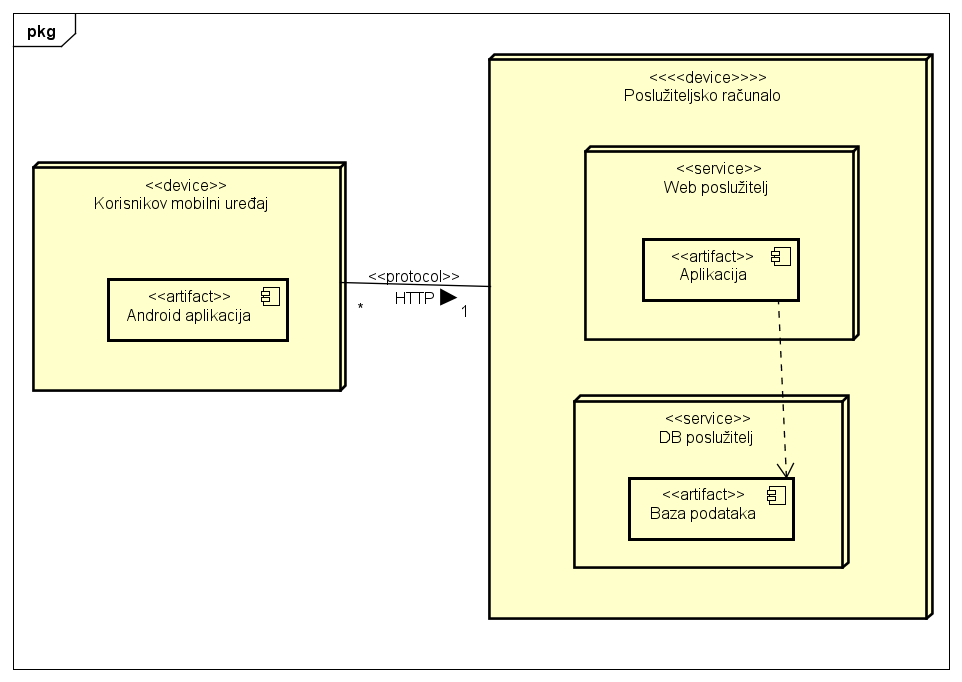
\includegraphics[scale=0.6]{dijagrami/dijagramRazmjestaja/dijagramRazmjestaja.PNG} %veličina slike u odnosu na originalnu datoteku i pozicija slike
			 	\centering
			 	\caption{Dijagram razmještaja}
			 	\label{fig:dRazmjestaja}
			 \end{figure}
			
			\eject 
		
		\section{Upute za puštanje u pogon}
		
			\textbf{\textit{dio 2. revizije}}\\
		
			...
			
			
			\eject 